%%%%%%%%%%%%%%%%%%%%%%%%%%%%%%%%%%%%%%%%%%%%%%%%%%%%%%%%%%%%%%%%%
% Projeto avaliativo da disciplina de programação 2
% Sub-projeto do grupo Doyle
%
% Autores:
%     Prof. Dr. Ruben Carlo Benante
%
%     Nome do Aluno 1
%     Thiago De Azevedo Cavendish
%     Nome do Aluno 3
%     Ulisses Mosart Sobrinho
%     Nome do Aluno 5
%     Nome do Aluno 6
%
% Data: 2021-11-08
%
% Assunto: escrever uma linha de explicação: Aulas sobre estruturas de controle de decisão
%
%%%%%%%%%%%%%%%%%%%%%%%%%%%%%%%%%%%%%%%%%%%%%%%%%%%%%%%%%%%%%%%%%

           % Geraçao do PDF %
%%%%%%%%%%%%%%%%%%%%%%%%%%%%%%%%%%%%%%%%%%%%%%%%%%%%%%%%%%%%%%%%%
% Para gerar o PDF use uma das 2 opções abaixo:
%
% Opção 1: com makefile
%    $ make pext-prog2-benante-sobrenome1-sobrenome2*.pdf
%
% Opção 2: comandos diretos:
%    $ pdflatex pext-matdiscreta-benante-sobrenome1-sobrenome2.tex -o pext-matdiscreta-benante-sobrenome1-sobrenome2.pdf
%    $ bibtex biblio 
%    $ pdflatex pext-matdiscreta-benante-sobrenome1-sobrenome2.tex -o pext-matdiscreta-benante-sobrenome1-sobrenome2.pdf

% preambulo %%%%%%%%%%%%%%%%%%%%%%%%%%%%%%%%%%%%%%%%%%%%%%%%%%%%%%
\documentclass[a4paper,10pt]{article}  % Duas colunas
\usepackage[utf8]{inputenc}  % letras acentuadas
\usepackage[portuguese]{babel}  % tradução de títulos
\usepackage{algorithm}  % ambiente para índice de algoritmos
\usepackage{algpseudocode}  % fonte e estilo do algoritmo
\usepackage{graphicx}
\usepackage{indentfirst}
% \usepackage{natbib}
%[noend]

\floatname{algorithm}{Algoritmo} % tradução da palavra algorítimo no ambiente de índice

%% Capa %%%%%%%%%%%%%%%%%%%%%%%%%%%%%%%%%%%%%%%%%%%%%%%%%%%%%%

\title{ Programação 2: 
        Aulas sobre estruturas de controle de decisão}

\author{Ruben Carlo Benante \\ Autor1 \\ Thiago De Azevedo Cavendish \\ Autor3 \\ Ulisses Mosart Sobrinho \\ Autor5 \\ Autor6 }

\begin{document} % início do PDF %

\maketitle

%% Resumo %%%%%%%%%%%%%%%%%%%%%%%%%%%%%%%%%%%%%%%%%%%%%%%%%%%%%%

\begin{abstract}

\textbf{Assunto:} Ensino de estruturas de controle de dicisão, da Linguagem de Programação \texttt{C}.

 Vamos comparar os algoritmos de estruturas de controle de decisão % \textit{xsort} e \textit{ysort} para bla bla.
% descrever em poucas palavras seu projeto aqui 

\textbf{Local:} Escola Politécnica de Pernambuco - UPE/POLI

\textbf{Órgão Financiador:} N/A

\textbf{Caracterização:} Projeto requisito da disciplina de Programação 2, sub-projeto do grupo \texttt{Doyle}

% Este é o fim do resumo.

\end{abstract}


% Artigos %%%%%%%%%%%%%%%%%%%%%%%%%%%%%%%%%%%%%%%%%%%%%%%%%%%%%%

%% seção de introdução %%%%%%%%%%%%%%%%%%%%%%%%%%%%%%%%%%%%%%%%%%%%%%%%%%%%%%

\section{Introdução}

% Descrever melhor seu projeto aqui 

   Esse projeto será composto de duas vídeo aulas sobre o tópico de ensino de estruturas de controle de decisão,  da Linguagem de Programação \texttt{C}

\begin{itemize}

 \item Estrutura de decisão If/Else
 \item Estrutura de controle Switch
\end{itemize}


 \subsection{Função básica}
% As estruturas de decisão If/Else tem como principal função ...


    Nós utilizamos as estruturas de decisão (If/Else) quando existem instruções
dentro do programa que só devem ser executadas se elas satisfizerem  
determinadas condições.


  .
  .  Por exemplo :

\begin{itemize}
               
       \item  Só irei para a praia se não chover. 
       \item  Só passarei nesta disciplina se eu obtiver uma média igual ou superior a 7,0 e se a presença for superior ou igual a 70 por cento das aulas.
             
\end{itemize}

   -  A sintaxe da estrutura IF na linguagem C é a seguinte :
 
 \subsection{Estrutura de Decisão IF}   
       
  -  Comando IF = se


\begin{table}
\begin{center}
 \caption{Tabela para melhor vizualização da estrutura do If}
\begin{tabular}{|l|r|}
  \hline \hline
  
  .          & if(condição) \\ \hline
  Estrutura  & chave 1  \\ \hline
    básica   &   lista de instruções  \\ \hline
  .          & chave 2  \\ \hline
  
\end{tabular}
\label{tab:resultados}
\end{center}
\end{table}

  
   O algoritmo \textit{acima} trabalha da seguinte maneira :
 

   -  A condição é verificada a cada passagem pela estrutura IF. Se a condição for satisfeita (V), então a lista de instruções que se encontra\\ entre chaves será executada.

.

  Porém, Se a condição NÃO for satisfeita (F), então serão executadas as instruções existentes logo após o fechamento das chaves.
 
 \subsection{Else}
 \subsubsection{Sobre} % a ser ajustado o nome dessa sessao 

  
 \subsection{Switch}
 \subsubsection{Sobre} % a ser ajustado o nome dessa sessao
    
  A palavra switch, associando ao seu significado do inglês, é um comando que funciona como uma chave de seleção/interruptor, sendo capaz de acionar tanto uma como diversas escolhas.

  O switch case é um comando utilizado na construção de menus de escolhas(“cases”) para o usuário, o qual diante de um leque de opções, poderá decidir algum dos casos e assim obter uma resposta relativa ao caso selecionado.
 

  \subsubsection{Aplicações}
% \subsubsection{Primeira aplicação}

    O comando “switch(variável)” assemelha seu funcionamento a de conjuntos “if-else”, como demonstrado logo abaixo em um programa cuja principal finalidade é receber e atribuir valores para a variável “valor” e em seguida imprimir na tela uma resposta de acordo com o valor digitado:

 \begin{figure}[H]
 \centering
 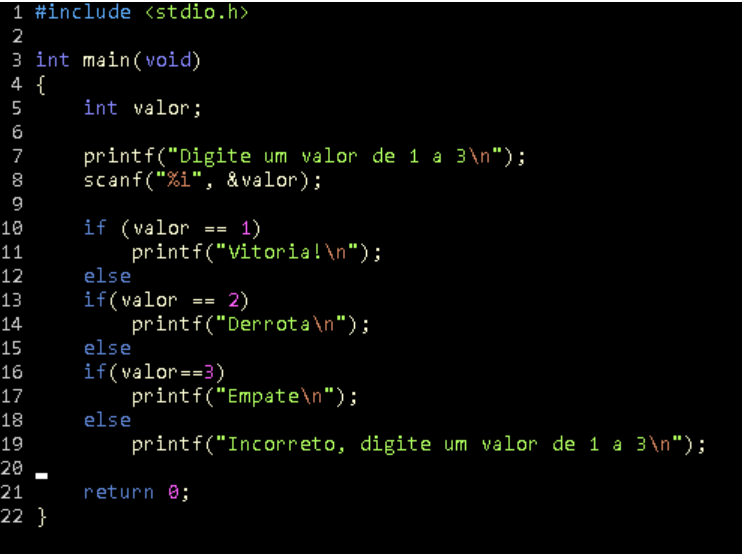
\includegraphics[width=.80\linewidth]{imagens/ex2.png}
 \caption{Exemplo de programa com alguns conjuntos de if-else}
 \label{fig:xsorta}
\end{figure}

    Assim como demonstrado acima, é possível criar uma sequência “if-else” em cadeia gerando um conjunto de casos que terão a mesma eficiência do comando switch, no entanto, caso o menu necessite diversos casos, o programa provavelmente ficará desorganizado e estará ocupando bastante espaço de maneira desnecessária. \par
     Agora, apresentando o mesmo programa, só que aplicando o conceito de “switch-case”, ficaria da seguinte maneira:

\begin{figure}[H]
 \centering
 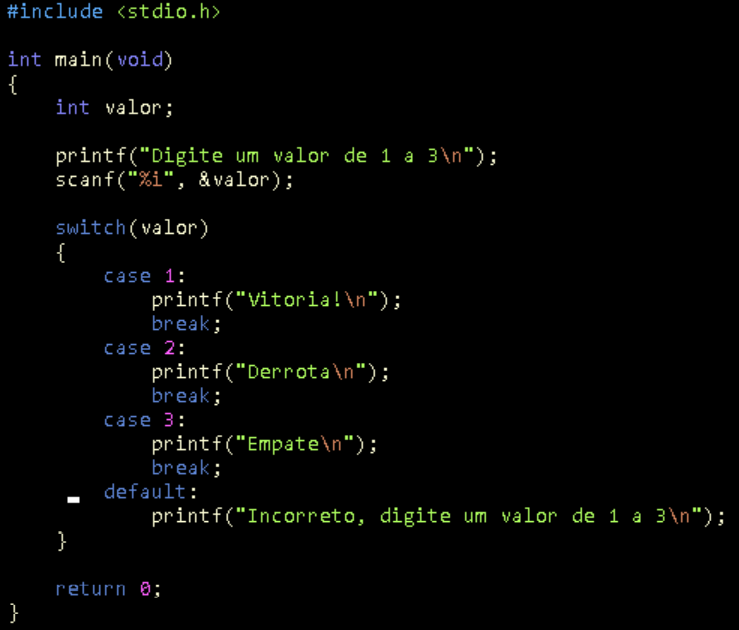
\includegraphics[width=.80\linewidth]{imagens/ex3.png}
 \caption{Aplicando o switch ao invés do if-else}
\end{figure}


 %\subsubsection{Segunda aplicação}

    Assim como o “if-else”, switch pode receber tanto um inteiro ou caractere como variável, exemplificado no programa a seguir:

\begin{figure}[H]
 \centering
 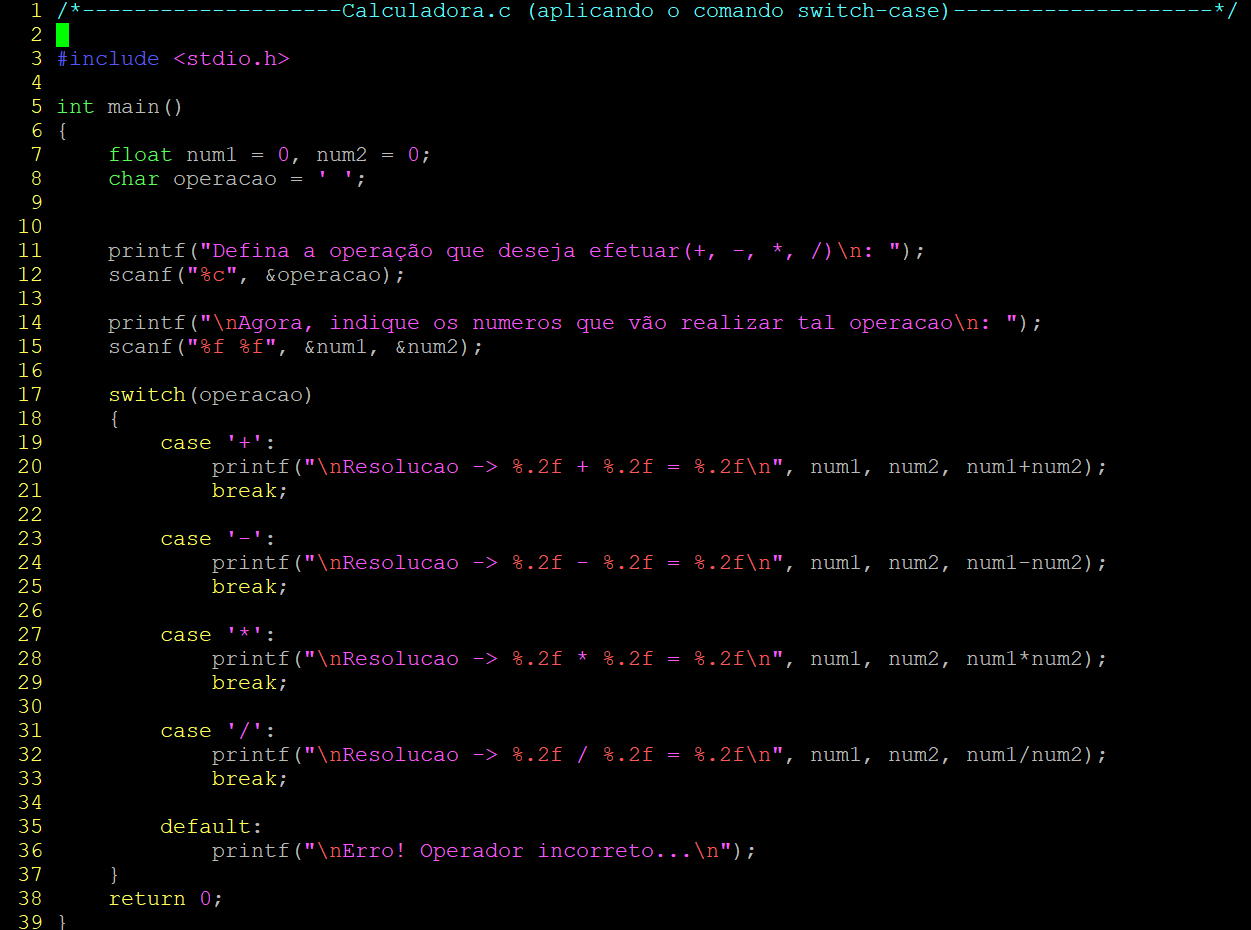
\includegraphics[width=.80\linewidth]{imagens/ex4.png}
 \caption{Calculadora} %fique a vontade para alterar o nome da imagem guilherme
 \label{fig:xsort}
\end{figure}

    O programa aproveita da praticidade do comando “switch(variável)”, simplificando toda a complexidade que necessitária de vários “if...else” encadeados. \par
 Nessa calculadora, o usuário deverá digitar a operação seguida dos números a fim de realizar o cálculo em questão: 
 
 \begin{figure}[H]
 \centering
 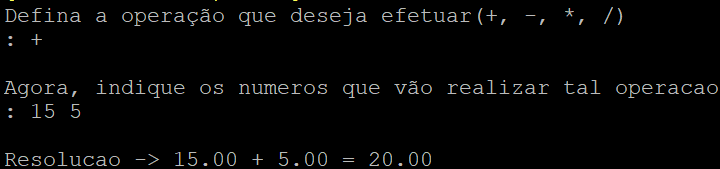
\includegraphics[width=.80\linewidth]{imagens/ex5.png}
 \caption{Operação de soma}
 \end{figure}

 \begin{figure}[H]
 \centering
 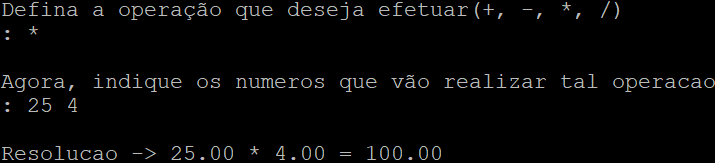
\includegraphics[width=.80\linewidth]{imagens/ex6.png}
 \caption{Operação de multiplicação}
\end{figure}

     A instrução “break” no código termina a execução do switch, evitando testar os demais comandos possíveis de forma desnecessária. \par
 O comando “default” serve para exibir uma mensagem caso nenhuma das operações anteriores tenham sido devidamente declaradas:


 \begin{figure}[H]
 \centering
 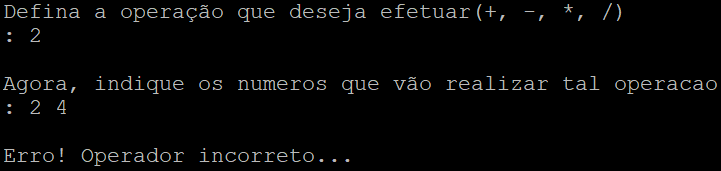
\includegraphics[width=.80\linewidth]{imagens/ex7.png}
 \caption{Operação indefinida}
\end{figure}


%% seção de objetivos %%%%%%%%%%%%%%%%%%%%%%%%%%%%%%%%%%%%%%%%%%%%%%%%%%%%%%
\section{Objetivos}

 \subsection{Objetivo Geral}

 Descrever o objetivo geral a ser alcançado

 \subsection{Objetivos Específicos}

Listar os objetivos específicos

\begin{itemize}
 \item Proporcionar tal e tal
 \item Realizar tal e tal
\end{itemize}


%% seção de justificativa %%%%%%%%%%%%%%%%%%%%%%%%%%%%%%%%%%%%%%%%%%%%%%%%%%%%%%
\section{Justificativa}

 Justificar seu projeto ...

%\begin{figure}[ht]
%\centering
%\includegraphics[width=.80\linewidth]{imagens/exemplo.png}
%\caption{Exemplo de ordenação com Bubblesort}
%\label{fig:xsort}
%\end{figure}


%% seção de metodologia %%%%%%%%%%%%%%%%%%%%%%%%%%%%%%%%%%%%%%%%%%%%%%%%%%%%%%
\section{Metodologia}

  Descrever como (por quais métodos) os objetivos serão alcançados.

   Esse projeto será composto de duas vídeo aulas sobre o tópico de ensino da Linguagem de Programação \texttt{C}

\begin{itemize}

 \item Aula sobre as estruturas de decisão If e Else
 \item Aula sobre a estrutura de controle Switch
\end{itemize}


  O algoritmo é descrito abaixo:


% subseção equipamentos %%%%%%%%%%%%%%%%%%%%%%%%%%%%%%%%%%%%%%%%%%%%%%%%%%%%%%
 \subsection{Equipamentos Necessários}

% Listar os equipamentos necessários para a implementação do projeto.

 Para realizar este projeto é preciso ter um computador, acesso à internet e tempo ...


% O método \emph{Ysort} é caracterizado por...

 % subseção com algoritmo %%%%%%%%%%%%%%%%%%%%%%%%%%%%%%%%%%%%%%%%%%%%%%%%%%%%%%
 \subsection{Implementação}

 Para conseguir blablabla


 O algoritmo \textit{Ysort} segue abaixo:

\begin{algorithm}
\caption{Algoritmo Ysort}\label{alg:ysort}
\begin{algorithmic}[1]
\Function{ysort}{estado}\Comment{retorna uma ação}
\State \textbf{Entradas}: estado é a configuração atual do jogo
\State $v\gets \mathrm{maxvalor}{(estado)}$
\State \textbf{returna} a ação $a$ em sucessores(estado) cujo valor é $v$ %\Comment{comentario}
% \While{$r\not=0$}\Comment{We have the answer if r is 0}
% \State $a\gets b$
% \State $b\gets r$
% \State $r\gets a\bmod b$
% \EndWhile\label{euclidendwhile}
\EndFunction
\Function{maxvalor}{estado}\Comment{retorna o valor estático}
\If{fim(estado)}
   \State \textbf{retorna} estatico(estado)
\EndIf
\State $v \gets -\infty$
\For{todas ações $a$ nos sucessores(estado)}
    \State $v \gets \max{(v, \mathrm{minvalor}(a))}$
\EndFor
\State \textbf{retorna} $v$
\EndFunction
\Function{minvalor}{estado}\Comment{retorna o valor estático}
\If{fim(estado)}
   \State \textbf{retorna} estatico(estado)
\EndIf
\State $v \gets \infty$
\For{todas ações $a$ nos sucessores(estado)}
    \State $v \gets \min{(v, \mathrm{maxvalor}(a))}$
\EndFor
\State \textbf{retorna} $v$
\EndFunction
\end{algorithmic}
\end{algorithm}


%% seção Plano de Trabalho %%%%%%%%%%%%%%%%%%%%%%%%%%%%%%%%%%%%%%%%%%%%%%%%%%%%%%
\section{Plano de Trabalho}

Esta seção estabelece as atividades a serem realizadas.


% seção Plano de Trabalho / Cronograma %%%%%%%%%%%%%%%%%%%%%%%%%%%%%%%%%%%%%%%%%%%%%%%%%%%%%%
\section{Cronograma}

   Em conjunto com a seção de Plano de Trabalho, a seção de cronograma coloca as atividades dispostas numa linha do tempo.


   Utilize uma tabela para melhor visualização.

\begin{table}
\begin{center}
 \caption{Tabela de custo de pontos para habilidades}
\begin{tabular}{|l|r|}
  \hline \hline
  pontos & moedas \\ \hline \hline
   8 & 0 \\ \hline
   9 & 1 \\ \hline
  10 & 2 \\ \hline
  11 & 3 \\ \hline
  12 & 4 \\ \hline
  13 & 5 \\ \hline
  14 & 7 \\ \hline
  15 & 9 \\ \hline \hline
\end{tabular} 
\label{tab:resultados}
\end{center}
\end{table}


%% seção de impactos alcançados %%%%%%%%%%%%%%%%%%%%%%%%%%%%%%%%%%%%%%%%%%%%%%%%%%%%%%
\section{Impactos alcançados } % e Transferências

 % subseção de impacto científico %%%%%%%%%%%%%%%%%%%%%%%%%%%%%%%%%%%%%%%%%%%%%%%%%%%%%%
 \subsection{Impacto Científico}

 Não há impacto científico relevante.

 % subseção de impacto tecnológico %%%%%%%%%%%%%%%%%%%%%%%%%%%%%%%%%%%%%%%%%%%%%%%%%%%%%%
 \subsection{Impacto Tecnológico}

 Não há impacto tecnológico relevante.

 % subseção de econônimo %%%%%%%%%%%%%%%%%%%%%%%%%%%%%%%%%%%%%%%%%%%%%%%%%%%%%%
 \subsection{Impacto Econômico}

 Não há impacto econômico relevante.

 % subseção de impacto social %%%%%%%%%%%%%%%%%%%%%%%%%%%%%%%%%%%%%%%%%%%%%%%%%%%%
 \subsection{Impacto Social}

   O projeto visa contribuir com o aprendizado das futuras geraçoes da sociedade de forma que... bla ... bla... blal


 % subseção de impacto ambiental %%%%%%%%%%%%%%%%%%%%%%%%%%%%%%%%%%%%%%%%%%%%%%%%%%%%%%
 \subsection{Impacto Ambiental}

Não há impacto ambiental relevante.

%% seção de Conclusão %%%%%%%%%%%%%%%%%%%%%%%%%%%%%%%%%%%%%%%%%%%%%%%%%%%%%%%%%%%%
\section{Conclusão}

.

   -  O Grupo Doyle terá como objetivo na execução dessas aulas ensinar o controle de decisão, da linguagem C, aos discentes interessados.
 Contará com sua exposição de ensino gravada que será disponibilizada e a elaboração de relatórios a fim de cumprir com os aspectos estabelecidos no Plano de Trabalho.

 % subconclusão %%%%%%%%%%%%%%%%%%%%%%%%%%%%%%%%%%%%%%%%%%%%%%%%%
%%%%%
 \subsection{Concluindo}


  O que mais o seu projeto agrega? O que é transferido? De onde vem? Para onde vai?


%% seção de resultados esperados %%%%%%%%%%%%%%%%%%%%%%%%%%%%%%%%%%%%%%%%%%%%%%%%%%%%%%
\section{Resultados Esperados}

Os resultados mostrados na tabela \ref{tab:resultados} demonstram ...


    Concluimos,com base nos estudos e testes coletados sobre os algoritmos de ordenação propostos, que para fins educacionais, o algoritmo \textit{BubbleSort} é mais indicado devido a sua simples implementação, cabendo então para o \textit{QuickSort} ser o mais indicado entre os dois, quando requer uma demanda em menor tempo e com mais eficiência.
.

- De acordo com \cite{Benante2008phd} e este é o fim do artigo.


%%%%%%%%%%%%%%%%%%%%%%%%%%%%%%%%%%%%%%%%%%%%%%%%%%%%%%%%%%%%%%%%%%%%%%%%%%%%%%%%%%%%%%%%%%%%%%%%%%%%%%%%%%%%
% referências bibliográficas %%%%%%%%%%%%%%%%%%%%%%%%%%%%%%%%%%%%%%%%%%%%%%%%%%%%%%
\section*{Referências Bibliográficas}

% cite todos, mesmo os não referenciados %%%%%%%%%%%%%%%%%%%%%%%%%%%%%%%%%%%%%%%%%%%%%%%%%%%%%%
\nocite{*}

% se necessario %%%%%%%%%%%%%%%%%%%%%%%%%%%%%%%%%%%%%%%%%%%%%%%%%%%%%%
% troca autor and autor por autor & autor, na bibliografia. O dcu usa "and"
%\renewcommand{\harvardand}{\&} % troca and pro &. O dcu usa "and"

% Estilos de bibliografia %%%%%%%%%%%%%%%%%%%%%%%%%%%%%%%%%%%%%%%%%%%%%%%%%%%%%%
% \bibliographystyle{abnt-alf} % Estilo alfabético da ABNT. Opção [num] para estilo numérico
%\bibliographystyle{apalike}
%\bibliographystyle{dcu} %citacao como (autor and autor, ano). Parece apalike. Rev. Control. Automacao. Use com harvard
%\bibliographystyle{agsm} % padrao harvard fica (autor & autor ano).
\bibliographystyle{acm}

% arquivo de banco de dados das referências %%%%%%%%%%%%%%%%%%%%%%%%%%%%%%%%%%%%%%%%%%%%%%%%%%%%%%
% renomear para o número do exercício correto
% o arquivo de bibliografia pode se chamar qualquer coisa, isso não muda o comando de gerar o PDF. 
% Por exemplo para 'mybiblio.bib', use \bibliography{mybiblio} e os comandos pdflatex e bibtex continuam os mesmos identicos com exN.
\bibliography{biblio}

\end{document}
